% !TeX program = lualatex
% !TeX encoding = utf8
% !TeX spellcheck = uk_UA
% !TeX root =../LabWork.tex

\part{Поляризація світла}

\nocite{akhmanov, Godzhaev}
\printbibliography[title={Рекомендована література}, heading=subbibliography]

\section{Означення}

Світлові хвилі є електромагнітними, тому вони поперечні. Наприклад, радіохвилі, що випромінюються штирьовою антеною у хвильовій зоні мають вигляд, зображений на рис~\ref{fig:linearPolarisation}. 

\begin{figure}[!h]\centering
% Electromagnetic wave - colored
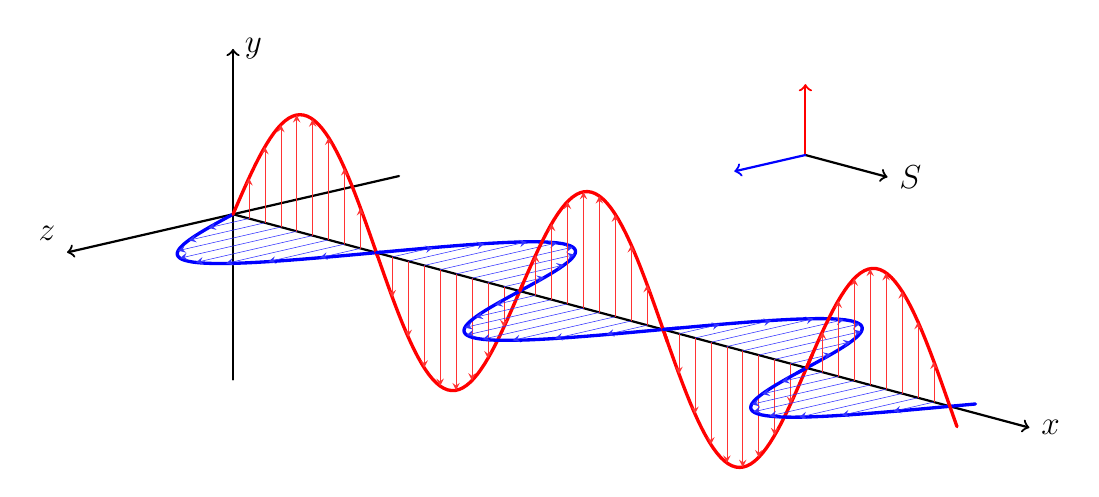
\begin{tikzpicture}[x=(-15:1.2), y=(90:1.0), z=(-150:1.0),
                    line cap=round, line join=round,
                    axis/.style={black, thick,->},
                    vector/.style={>=stealth,->}]
  \large
  \def\A{1.5}
  \def\nNodes{5} % use even number
  \def\nVectorsPerNode{8}
  \def\N{\nNodes*40}
  \def\xmax{\nNodes*pi/2*1.01}
  \pgfmathsetmacro\nVectors{(\nVectorsPerNode+1)*\nNodes}
 
 
  \def\drawENode{ % draw E node and vectors with some offset
    \draw[red,very thick,variable=\t,domain=\iOffset*pi/2:(\iOffset+1)*pi/2*1.01,samples=40]
      plot (\t,{\A*sin(\t*360/pi)},0);
    \foreach \k [evaluate={\t=\k*pi/2/(\nVectorsPerNode+1);
                           \angle=\k*90/(\nVectorsPerNode+1);}]
                in {1,...,\nVectorsPerNode}{
      \draw[vector, help lines, red!80]  (\iOffset*pi/2+\t,0,0) -- ++(0,{\A*sin(2*\angle+\iOffset*180)},0);
    }
  }
  \def\drawBNode{ % draw B node and vectors with some offset
    \draw[blue,very thick,variable=\t,domain=\iOffset*pi/2:(\iOffset+1)*pi/2*1.01,samples=40]
      plot (\t,0,{\A*sin(\t*360/pi)});
    \foreach \k [evaluate={\t=\k*pi/2/(\nVectorsPerNode+1);
                           \angle=\k*90/(\nVectorsPerNode+1);}]
                in {1,...,\nVectorsPerNode}{
      \draw[vector,help lines, blue!80]  (\iOffset*pi/2+\t,0,0) -- ++(0,0,{\A*sin(2*\angle+\iOffset*180)});
    }
  }
 
  % main axes
  \draw[axis] (0,0,0) -- ++(\xmax*1.1,0,0) node[right] {$x$};
  \draw[axis] (0,-\A*1.4,0) -- (0,\A*1.4,0) node[right] {$y$};
  \draw[axis] (0,0,-\A*1.4) -- (0,0,\A*1.4) node[above left] {$z$};
 
  % small axes
  \def\xOffset{{(\nNodes-2)*pi/2}}
  \def\yOffset{\A*1.2}
  \def\zOffset{\A*1.2}
  \draw[axis,black] (\xOffset,\yOffset,-\zOffset) -- ++(\A*0.6,0,0) node[right,align=center] {$\vect{S}$}; %\\propagation
  \draw[axis,red]  (\xOffset,\yOffset,-\zOffset) -- ++(0,\A*0.6,0) node[right] {$\Efield$};
  \draw[axis,blue]   (\xOffset,\yOffset,-\zOffset) -- ++(0,0,\A*0.6) node[above left] {$\Bfield$};
 
  % equation

 
  % draw (anti-)nodes
  \foreach \iNode [evaluate={\iOffset=\iNode-1;}] in {1,...,\nNodes}{
    \ifodd\iNode \drawBNode \drawENode % E overlaps B
    \else        \drawENode \drawBNode % B overlaps E
    \fi
  }
 
\end{tikzpicture}
%  \begin{tikzpicture}[x={(-10:1cm)},y={(90:1cm)},z={(210:1cm)},>={stealth}]
%    % Axes
%    \draw (-1,0,0) node[above] {$x$} -- (5,0,0);
%    \draw[-latex] (0,0,0) -- (0,2,0) node[above] {$y$};
%    \draw[-latex] (0,0,0) -- (0,0,2) node[left] {$z$};
%    % Propagation
%    \draw[->,ultra thick] (5,0,0) -- node[above] {$c$} (6,0,0);
%    % Waves
%    \draw[thick, red] plot[domain=0:4.5,samples=200] (\x,{cos(deg(pi*\x))},0);
%    \draw[gray,thick,blue] plot[domain=0:4.5,samples=200] (\x,0,{cos(deg(pi*\x))});
%    % Arrows
%    \foreach \x in {0.1,0.3,...,4.4} {
%      \draw[->,help lines, red] (\x,0,0) -- (\x,{cos(deg(pi*\x))},0);
%      \draw[->,help lines, blue] (\x,0,0) -- (\x,0,{cos(deg(pi*\x))});
%    }
%    % Labels
%    \node[above right] at (0,1,0) {$\Efield$};
%    \node[below] at (0,0,1) {$\Bfield$};
%  \end{tikzpicture}
\caption{Лінійно поляризоване світло}
\label{fig:linearPolarisation}
\end{figure}

При розгляді таких явищ, як поляризація світла, зазвичай всі міркування пов'язують з площиною коливань вектора напруженості електричного поля $\Efield$~--- світлового вектора, так як хімічний, фізіологічний та інші види впливу світла на речовину обумовлені головним чином електричними коливаннями. Однак при цьому слід пам'ятати про обов'язкове існування перпендикулярного йому вектора напруженості магнітного поля $\Bfield$.

На відміну від електромагнітної хвилі, що випромінюється антеною, світло випромінюється тілами і складається з хвиль, які випускають його окремі атоми. Випромінювання окремого атома триває близько $10^{-8}$~с і являє собою, як кажуть, цуг хвиль довжиною в середньому близько $3$~м. Випромінюючи, атом через деякий час, прийшовши в збуджений стан, випромінює знову і так повторюється знову. Одночасно випромінює безліч атомів. Породжені ними цуги хвиль, накладаючись один на одного, утворюють світлову хвилю. Напрями коливань для кожного цуга орієнтовані випадковим чином. Тому в результуючій світловій хвилі коливання світлового вектора відбуваються в різних напрямках з однаковою ймовірністю. Це треба розуміти так, що при проходженні світлової хвилі через деяку точку коливання світлового вектора швидко і безладно змінюють один одного. Але в межах деякого короткого часу ми маємо справу зі світловим вектором, напрямок коливань якого зберігається, потім напрямок коливань змінюється на інший і т. д. 



При це модуль світлового вектора залишається незмінним.  Таке світло називають \emph{природним}. Умовно це зображують як на рис.~\ref{fig:NonPolarisation}. Світло, в якому напрям коливань світлового вектора упорядкований якимось чином, називають поляризованим. Якщо коливання світлового вектора відбуваються тільки в одній площині, світло називають плоско (або лінійно) поляризованим, так, як це показано на рис.~\ref{fig:linearPolarisation}. Якщо кінець світлового вектора описує еліпс, то такий світло називають еліптично-поляризованим (зокрема, поляризованим по колу, рис.~\ref{fig:CircularPolarisation}).



\begin{figure}[!h]\centering
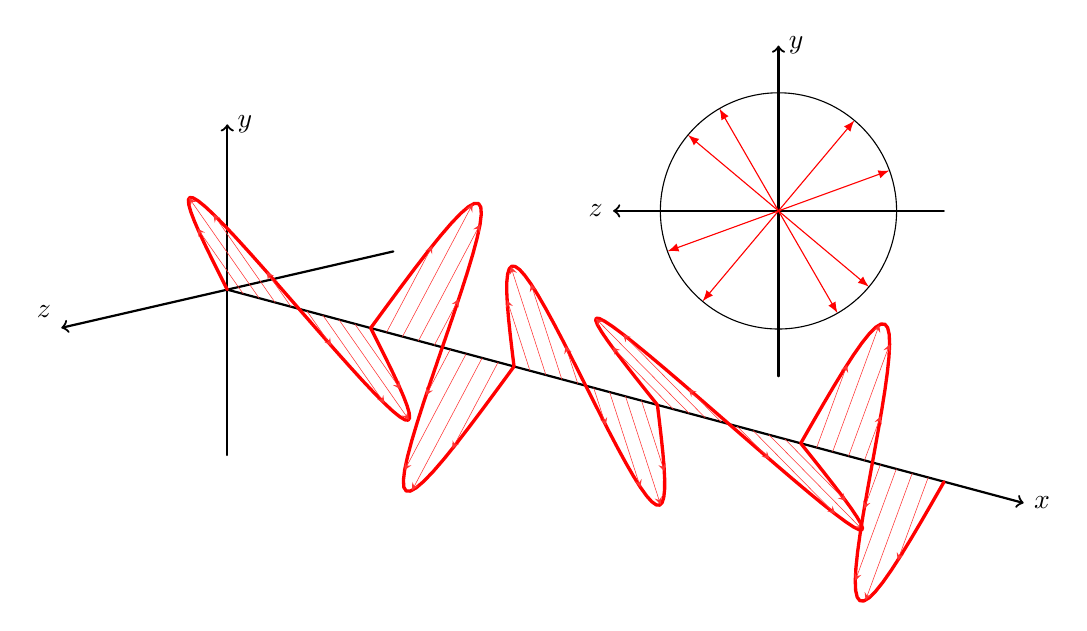
\begin{tikzpicture}[coord/.style={x=(-15:1.2), y=(90:1.0), z=(-150:1.0)},
                    line cap=round, line join=round,
                    axis/.style={black, thick,->},
                    vector/.style={>=stealth,->}]
%  \large
  \def\A{1.5}
  \def\nNodes{5} % use even number
  \def\nVectorsPerNode{8}
  \def\N{\nNodes*40}
  \def\xmax{\nNodes*pi/2*1.01}
  \pgfmathsetmacro\nVectors{(\nVectorsPerNode+1)*\nNodes}
 
 
  \def\drawENode#1{ % draw E node and vectors with some offset
    \draw[coord, red,very thick,variable=\t,domain=\iOffset*pi/2:(\iOffset+1)*pi/2*1,samples=40]
      plot (\t,{\A*sin(4*deg(\t))},{#1*\A*sin(4*deg(\t))});
  \foreach \k [evaluate={\t=\k*pi/2/(\nVectorsPerNode+1);
                           \angle=\k*90/(\nVectorsPerNode+1);}]
                in {1,...,\nVectorsPerNode}{
      \draw[coord, vector, help lines, red!80]  (\iOffset*pi/2+\t,0,0) -- ++(0,{\A*sin(4*deg(\t))},{#1*\A*sin(4*deg(\t))});
    }
  }

 
  % main axes
  \draw[axis, coord] (0,0,0) -- ++(\xmax*1.1,0,0) node[right] {$x$};
  \draw[axis, coord] (0,-\A*1.4,0) -- (0,\A*1.4,0) node[right] {$y$};
  \draw[axis, coord] (0,0,-\A*1.4) -- (0,0,\A*1.4) node[above left] {$z$};
 
  % small axes
  \def\xOffset{{(\nNodes-2)*pi/2}}
  \def\yOffset{\A}
  \def\zOffset{\A}
   \coordinate (O) at (7,1); 
%  \draw[axis,black] (\xOffset,\yOffset,-\zOffset) -- ++(\A*0.6,0,0) node[right,align=center] {$e$}; 
    \draw[axis]  (O) -- +(-90:\A*1.4) -- +(90:\A*1.4) node[right] {$y$};
    \draw[axis]  (O) --  +(0:\A*1.4) -- +(180:\A*1.4) node[left] {$z$};

  \draw[-latex,red]  (O) -- +(-60:\A);
  \draw[-latex,red]  (O) -- +(120:\A);

  \draw[-latex,red]  (O) -- +(-130:\A);
  \draw[-latex,red]  (O) -- +(50:\A);

  \draw[-latex,red]  (O) -- +(-40:\A);
  \draw[-latex,red]  (O) -- +(140:\A);

  \draw[-latex,red]  (O) -- +(-160:\A);
  \draw[-latex,red]  (O) -- +(20:\A);

%     \draw[axis,red]  (7,2) -- ++(180-120:\A);
  \draw[black]  (O) circle (\A);

 
  % draw (anti-)nodes
\def\iOffset{0} \drawENode{0.6}
\def\iOffset{1} \drawENode{-0.6}
\def\iOffset{2} \drawENode{0.3}
\def\iOffset{3} \drawENode{0.8}
\def\iOffset{4} \drawENode{-0.4}
\end{tikzpicture}
\caption{Неполяризоване (природне) світло}
\label{fig:NonPolarisation}
\end{figure}



\begin{figure}[!h]\centering
% Electromagnetic wave - circular polarization
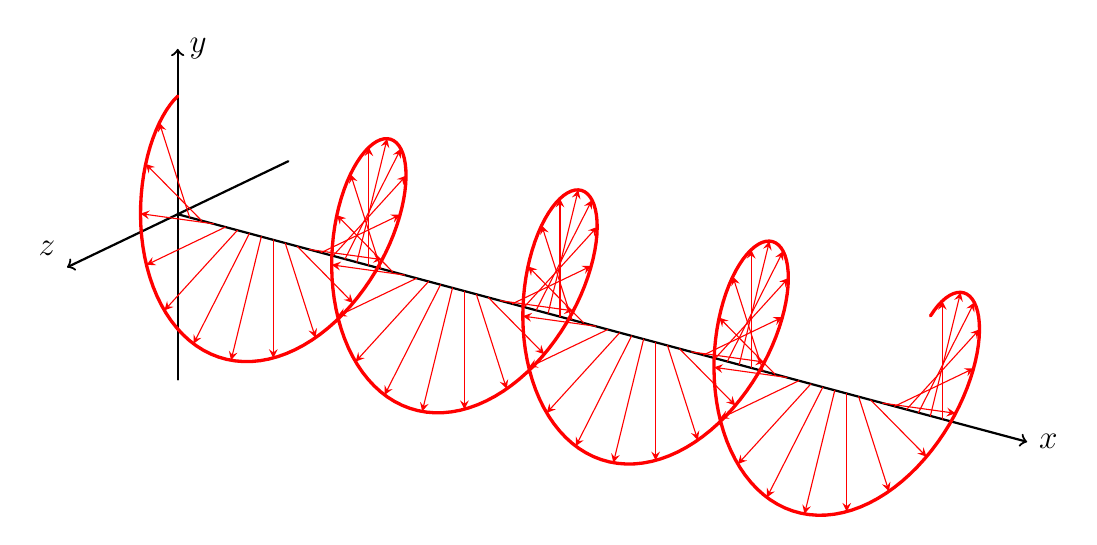
\begin{tikzpicture}[x=(-15:0.8), y=(90:1.0), z=(-150:1.0),
                    line cap=round, line join=round,
                    axis/.style={black, thick,->},
                    vector/.style={>=stealth,->}]
  \large
  \def\A{1.5}
  \def\nNodes{8} % use even number
  \def\nVectorsPerNode{8}
  \def\N{\nNodes*40}
  \def\xmax{\nNodes*pi/2*1.01}
  \pgfmathsetmacro\nVectors{\nVectorsPerNode*\nNodes}
 
 
  % main axes
  \draw[axis] (0,0,0) -- ++(\xmax*1.1,0,0) node[right] {$x$};
  \draw[axis] (0,-\A*1.4,0) -- (0,\A*1.4,0) node[right] {$y$};
  \draw[axis] (0,0,-\A*1.4) -- (0,0,\A*1.4) node[above left] {$z$};
 
  % waves
  \draw[red,very thick,variable=\t,domain=0:\nNodes*pi/2*1.01,samples=\N]
    plot (\t,{\A*cos(\t*360/pi)},{\A*sin(\t*360/pi)});
 
  % draw vectors
  \foreach \k [evaluate={\t=\k*pi/2/\nVectorsPerNode;
                         \angle=\k*90/\nVectorsPerNode;}]
              in {1,...,\nVectors}{
    \draw[vector, red] (\t,0,0) -- ++(0,{\A*cos(2*\angle)},{\A*sin(2*\angle)});
  }
 
\end{tikzpicture}
\caption{Світло, поляризоване по колу}
\label{fig:CircularPolarisation}
\end{figure}

З природного світла можна отримати плоскополяризоване за допомогою приладів, які називаються поляризаторами. Ці прилади вільно пропускають коливання світлового вектора, паралельні площині, яку ми будемо називати площиною пропускання поляризатора. Коливання ж, перпендикулярні до цієї площини, затримуються повністю або частково. У першому випадку поляризатор є ідеальним.

Крім плоскополяризованого і природного світла існує ще <<проміжний>> випадок ---
це частково-поляризоване світло. Частково-поляризоване світло, як і природне, можна представити у вигляді накладення
двох некогерентних плоскополяризованих хвиль з взаємно перпендикулярними площинами поляризації, але різними за інтенсивністю. Його також можна розглядати як суміш природною  і плоскополяризованого складових.

Частково-поляризоване світло характеризують ступенем поляризації $P$, яку визначають як:
\begin{equation}\label{eq: PolarizationLevel}
    P = \frac{I_{\max} - I_{\min}}{I_{\max} + I_{\min}} = \frac{I_\text{пол}}{I_0},
\end{equation}
де $I_0 = I_{\max} + I_{\min}$~--- інтенсивність падаючого на аналізатор світла, $I_\text{пол}$~--- інтенсивність поляризованої компоненти світла. 

Для плоскополяризованого світла $I_\text{пол} = I_0$, а тому ступінь поляризації $P = 1$, для природного світла $I_\text{пол} = 0$, тому  $P = 0$. Це два крайніх випадки. Однак,  що для еліптично-поляризованого світла поняття <<ступінь поляризації>> не застосовне, а тому і формула~\eqref{eq: PolarizationLevel} також не застосовна.

\subsection{Закон Малюса}

Поляризатори можна використовувати і в якості аналізаторів~--- для визначення характеру і ступеня поляризації світла.
Нехай на аналізатор падає лінійно-поляризоване світло, вектор $\Efield$ якого становить кут $\phi$ з площиною пропускання
поляризатора. Аналізатор пропускає тільки ту складову вектора $\Efield$, яка паралельна площині пропускання, тобто $\Efield_0 \cos\phi$ (рис.~\ref{label}). Інтенсивність пропорційна квадрату модуля світлового вектора, тому інтенсивність світла, яке пройшло аналізатор визначається за формулою:
\begin{equation}\label{eq:MaluseLow}
    I = I_0\cos^2\phi.
\end{equation}

\begin{figure}[!h]\centering
\colorlet{crystal}{blue!75}
\begin{tikzpicture}[coord/.style={x=(-15:1.2), y=(90:1.0), z=(-150:1.0)},
                    line cap=round, line join=round,
                    axis/.style={black, thick,->},
                    vector/.style={>=stealth,->},
                    plate/.style={coord, fill, opacity=0.875},]
%  \large
  \def\A{1.5}
  \def\nNodes{5} % use even number
  \def\nVectorsPerNode{8}
  \def\N{\nNodes*40}
  \def\xmax{\nNodes*pi/2*1.01}
  \pgfmathsetmacro\nVectors{(\nVectorsPerNode+1)*\nNodes}
 
 
  \def\drawENode#1#2{ % draw E node and vectors with some offset
    \draw[coord, red,very thick,variable=\t,domain=\iOffset*pi/2:(\iOffset+1)*pi/2,samples=40]
      plot (\t,{\A*#2*sin(4*deg(\t))},{#1*#2*\A*sin(4*deg(\t))});
  \foreach \k [evaluate={\t=\k*pi/2/(\nVectorsPerNode+1);
                           \angle=\k*90/(\nVectorsPerNode+1);}]
                in {1,...,\nVectorsPerNode}{
      \draw[coord, vector, help lines, red!80]  (\iOffset*pi/2+\t,0,0) -- ++(0,{\A*#2*sin(4*deg(\t))},{#1*#2*\A*sin(4*deg(\t))});
    }
  }

 
  % main axes
  \draw[axis, coord] (0,0,0) -- ++(\xmax*1.3,0,0) node[right] {$x$};
  \draw[axis, coord] (0,-\A*1.4,0) -- (0,\A*1.4,0) node[right] {$y$};
  \draw[axis, coord] (0,0,-\A*1.4) -- (0,0,\A*1.4) node[above left] {$z$};
 
  % small axes


 
  % draw (anti-)nodes
\def\iOffset{0} \drawENode{0.6}{1}
\def\iOffset{1} \drawENode{-0.6}{1}
\begin{scope}[xscale=2, yscale=2]
    \def\XOffset{1*pi/2}
    \path [crystal!25, plate] 
        (\XOffset,-1,-1) -- (\XOffset,-1,1) -- (\XOffset,1,1) -- (\XOffset,1,-1) -- cycle;
    \path [crystal!50, plate] 
        (\XOffset,-1,1) -- ({\XOffset-0.1},-1,1) -- ({\XOffset-0.1},1,1) -- (\XOffset,1, 1) -- 
        cycle;
    \path [crystal!75, plate] 
        (\XOffset,1,-1) -- ({\XOffset-0.1},1,-1) -- ({\XOffset-0.1},1,1) -- (\XOffset,1, 1) -- cycle;
    \draw[-latex, plate] (\XOffset,-1,0) -- (\XOffset,1,0) ;
    \draw[-latex, plate] (\XOffset,0,-1) -- (\XOffset,0,1) ;
%    \node [yslant=tan(\xangle), text=crystal!50, below, font=\small] at 
%        (-1,-1,0){Linear Polarizer};
\end{scope}
\def\iOffset{2} \drawENode{0}{0.6}
\def\iOffset{3} \drawENode{0}{0.6}

\begin{scope}[xscale=2, yscale=2]
    \def\XOffset{2*pi/2}
    \path [crystal!25, plate, rotate around={25:(\XOffset,0,0)}] (\XOffset,-1,-1) -- (\XOffset,-1,1) -- (\XOffset,1,1) -- (\XOffset,1,-1) -- cycle;
    \path [crystal!50, plate,rotate around={25:(\XOffset,0,0)}] 
        (\XOffset,-1,1) -- ({\XOffset-0.1},-1,1) -- ({\XOffset-0.1},1,1) -- (\XOffset,1, 1) -- 
        cycle;
    \path [crystal!75, plate, rotate around={25:(\XOffset,0,0)}] 
        (\XOffset,1,-1) -- ({\XOffset-0.1},1,-1) -- ({\XOffset-0.1},1,1) -- (\XOffset,1, 1) -- cycle;
    \draw[-latex, plate,dashed] (\XOffset,-1,0) -- (\XOffset,1,0) coordinate[pos=0.75] (A1);
    \draw[-latex, plate,dashed] (\XOffset,0,-1) -- (\XOffset,0,1) ;

    \draw[-latex, plate,rotate around={25:(\XOffset,0,0)}] (\XOffset,-1,0) -- (\XOffset,1,0) coordinate[pos=0.75] (A2) ;
    \draw[-latex, plate, rotate around={25:(\XOffset,0,0)}] (\XOffset,0,-1) -- (\XOffset,0,1) ;
    
    \draw[->] (A1) to[bend right] node[above] {$\phi$} (A2);

    \node [coord, yslant=tan(15), text=crystal!50, below, font=\small] at 
        (0.1,-1,0) {Не поляризоване світло};
    \node [coord, yslant=tan(15), text=crystal!50, below, font=\small] at 
        (2,-1,1.5) {Поляризоване, $I_0$};
    \node [coord, yslant=tan(15), text=crystal!50, below, font=\small] at 
        (4,-1,1.5) {Поляризоване, $I = I_0\cos^2\phi$};
\end{scope}
\def\iOffset{4} \drawENode{0.5}{0.4}
\def\iOffset{5} \drawENode{0.5}{0.4}
\end{tikzpicture}
\label{fig:MaluseLaw}
\caption{Проходження світла через систему <<поляризатор-аналізатор>>.}
\end{figure}

\subsection{Поляризація при відбиванні та заломленні світла. Кут Брюстера}

Якщо кут падіння природного світла на межу розділу двох прозорих діелектриків відмінний від нуля, то відбитий і заломлений пучки виявляються частково-поляризованими. У відбитому світлі переважають коливання вектора $\Efield$, перпендикулярні до площини падіння, а в переломленому світлі~--- паралельні площині падіння. Ступінь поляризації обох хвиль (відбитої і заломленої) залежить від кута падіння. При деякому значенні кута падіння відбите світло стає повністю поляризованим, і його площина поляризації (площина коливань вектора $\Efield$) виявляється перпендикулярною до площини падіння. Цей кут задовольняє наступній умові:
\begin{equation}\label{eq:BrusterLaw}
    \tg i_\text{Б} = \frac{n_2}{n_1}
\end{equation}

\begin{figure}[!h]\centering
\begin{tikzpicture}
\def\dotMarkRightAngle[size=#1](#2,#3,#4){%
 \draw ($(#3)!#1!(#2)$) -- 
       ($($(#3)!#1!(#2)$)!#1!90:(#2)$) --
       ($(#3)!#1!(#4)$);
}
        \coordinate (O) at (0,0);
%    	\draw (-3,-3) to [grid with coordinates] (3,3);
        \fill[cyan!50] (-3,-3) rectangle (3,0);
        \draw (0,-1) -- (0,1);
        \draw[latex-] (0,0) -- (90+55:3);
        \foreach \i in {0.1,0.2,...,0.9} {\draw[-latex] (0,0) -- (90-55:3) node[fill, circle ,draw=black,scale=0.25, pos=\i]  {} coordinate[pos=0.05] (A1);}
        \foreach \i in {0.1,0.3,...,0.8} {\draw[-latex] (0,0) -- (-90+35:3) node[fill, circle ,draw=black,scale=0.25, pos=\i]  {} 
        node[rotate=-8, draw, strike out, scale=0.9, pos=\i+0.05]  {} 
        node[rotate=-8, draw, strike out, scale=0.9, pos=\i+0.1]  {} 
        node[rotate=-8, draw, strike out, scale=0.9, pos=\i+0.15]  {}
        node[fill, circle ,draw=black,scale=0.25, pos=0.9]  {}  
        coordinate[pos=0.05] (A2) ;}
        \draw[stealth-] (0,0) ++(0,0.5)  arc(90:{90+55}:0.5)  node[pos=0.5, above] {$i_\text{Б}$} ;
        \dotMarkRightAngle[size=6pt](A1,O,A2);
        \node at (2.5,-0.5) {$n_2$};
        \node at (2.5,+0.5) {$n_1$};
	\end{tikzpicture}
\label{fig:Intermedia}
\caption{Падіння світла на границю розділу двох діелектриків}
\end{figure}

Можна переконатися, що при падінні світла під кутом Брюстера відбитий і заломлений промені взаємно ортогональні. При падінні природного світла під кутом Брюстера на межу розділу двох прозорих діелектриків заломлена хвиля стає частково-поляризованою, причому ступінь поляризації її виявляється максимальною.

Закон Брюстера є наслідком формул Френеля, які дають змогу розрахувати інтенсивності відбитого світла від межі розділу:
\begin{align}
    I_{\perp}^{\prime} &= I_{\perp}\frac{\sin^2(i - r)}{\sin^2(i + r)}, \\
    I_{\parallel}^{\prime} &= I_{\parallel}\frac{\tg^2(i - r)}{\tg^2(i + r)}, \label{eq:FrenselParallel}
\end{align}
де $i$~--- кут падіння, $r$~--- кут відбивання, $I_{\perp}$, $I_{\parallel}$~--- інтенсивності падаючого світла, $I_{\perp}^{\prime}$, $I_{\parallel}^{\prime}$~--- інтенсивності відбитого світла, індекси $\perp$ та $\parallel$ відповідають поляризації, перпендикулярній ($s$-поляризація) і паралельній ($p$-поляризація) площині падіння, відповідно.
